\documentclass[cmbright,doublespace]{WileySTAT-V1} 
%\documentclass[cmbright,doublespace,demo]{WileySTAT-V1} %% draft mode

\usepackage{verbatim}
\usepackage{statex2}
%\usepackage{shortvrb}

%\usepackage{mathtime}   %% Uses times
% mathtime free alternative: the newtx package
\usepackage[cmintegrals,cmbraces]{newtxmath}
 % do NOT use option varg: we want v's to look like v's
\usepackage[bookmarksopen,bookmarksnumbered,citecolor=blue,urlcolor=blue]{hyperref} %% Online requirements
\usepackage{natbib}     %% Used for Author Name and year
\usepackage{dcolumn}    %% For Tabular decimal alignments
\newcolumntype{d}[1]{D{.}{.}{#1}}

%% Journal informations \ref{}
\def\volumeyear{2019}
\def\volumenumber{99}
\def\DOI{ISBN.stat00999.pub9}

%% Set running heads
\runninghead{Rodney Sparapani and Robert McCulloch}{BART}

%% AMS Theorems
\newtheorem{theorem}{Theorem}
\newtheorem{proposition}[theorem]{Proposition} 
%% remove [theorem] for Unique numbering
\theoremstyle{plain}
\newtheorem{example}[theorem]{Example} 
%% remove [theorem] for Unique numbering
\newtheorem{definition}[theorem]{Definition} 
%% remove [theorem] for Unique numbering

\raggedbottom

\begin{document}

\title{Bayesian Additive Regression Trees (BART)}

\author{Rodney Sparapani\affil{a}\corrauth and
        Robert McCulloch\affil{b}}

\address{%
\affilnum{a}Medical College of Wisconsin, Milwaukee, WI, USA \\
\affilnum{b}Arizona State University, Tempe, AZ, USA}
\corremail{rsparapa@mcw.edu}

%%\articlenote{This is article note. }

\begin{abstract}
  This article introduces the nonparametric machine learning technique
  known as Bayesian Additive Regression Trees (BART) for continuous,
  dichotomous, categorical and time-to-event outcomes.
\end{abstract}

\keywords{black-box models; categorical outcomes; competing risks;
  continuous outcomes; dichotomous outcomes; ensemble predictive
  modeling; nonparametric; machine learning; recurrent events;
  survival analysis}

\maketitle

\section{Introduction}

Bayesian Additive Regression Trees (BART) arose out of earlier
research on Bayesian model fitting of an outcome to a single tree
\citep{ChipGeor98}; for more on approaches like this, see
\textbf{Classification and Regression Trees Methods} \citep{Loh14}
that carry the popular acronym CART.  In that era (circa 1998), the
outstanding predictive performance of ensemble models was starting to
become apparent
\citep{Brei96,KrogSoli97,FreuScha97,Brei01,Frie01,BaldBrun01}.
Instead of making a single prediction from a complex model, ensemble
models make a prediction which is the summary of the predictions from
many simple models.  Generally, ensemble models have desirable
properties, e.g., on the spectrum from low bias with high variance
(such as CART \citep{Brei17}) to high bias with low variance (linear
regression), ensemble models generally fall somewhere in the middle
which accounts for their superior performance \citep{KuhnJohn13}.
With some similarities to bagging \citep{Brei96}, boosting
\citep{FreuScha97,Frie01} and random forests \citep{Brei01}, BART
relies on an ensemble of trees to predict the outcome.

BART is a Bayesian nonparametric, sum of trees method for continuous,
dichotomous, categorical and time-to-event outcomes.  Furthermore,
BART is a black-box, machine learning method which fits the outcome
via an arbitrary random function, $f$, of the covariates.  So-called
black-box models generate functions of the covariates which are so
complex that interpreting the internal details of the fitted model is
generally abandoned in favor of assessment via evaluations of the
fitted function, $f$, at chosen values of the covariates
\citep{Frie01}.  As shown by \citet{ChipGeor10}, BART's out-of-sample
predictive performance is generally equivalent to, or exceeds that, of
alternatives like lasso with L1 regularization \citep{EfroHast04} or
black-box models such as gradient boosting \citep{FreuScha97,Frie01},
neural nets with one hidden layer \citep{Ripl07,VenaRipl13} and random
forests \citep{Brei01}.  \textbf{Overfitting (Overtraining)} is the
tendency to over-do the fit of a model to an in-sample training data
set's signal, and particularly its noise, resulting in poor predictive
performance for unseen out-of-sample data \citep{Cris14,CookRans16}.
Typically, BART does not over-fit to the training data due to the
regularization tree-branching penalty of the BART prior, i.e.,
generally, each tree in the ensemble has few branches and plays a
small part in the overall fit (see formula \eqref{regularity}
below). Essentially, BART is a Bayesian nonlinear model with all the
advantages of the Bayesian paradigm such as posterior inference
including point and interval estimation.  Conveniently, BART naturally
scales to large numbers of covariates and facilitates variable
selection; it does not require the covariates to be rescaled; neither
does it require the covariate functional relationship, nor the
interactions considered, to be pre-specified.

In this article, we will discuss the BART prior in the context of
continuous outcomes in Section~\ref{prior} along with posterior
computations in Section~\ref{post}.  In Section~\ref{Boston}, we
demonstrate BART with a classic example.  Next, we will briefly
discuss BART extensions for dichotomous, categorical and survival
outcomes in Section~\ref{gbart}.  We will then conclude with some
recent developments and software implementations (as of this writing)
in Section~\ref{final}.

\section{Binary trees and the BART prior}\label{prior}

Here, we briefly describe binary trees and their relationship to BART;
for a more detailed discussion of trees and tree-based methods, see
\textbf{Tree-structured Statistical Methods} \citep{ZhanCrow14}.  BART
relies on an ensemble of $H$ binary trees which are a type of a
directed acyclic graph.  For illustration, we fully exploit
the wooden tree metaphor with binary trees.  Each of these trees grows
from the ground up starting out as a root node.  The root node is
generally a branch decision rule, but it doesn't have to be;
occasionally there are trees in the ensemble which are only a root
terminal node consisting of a single leaf output value.  If the root
is a branch decision rule, then it spawns a left and a right node
which each can be either a branch decision rule or a terminal leaf
value and so on.  In binary tree, $\mathcal{T}$, there are $C$ nodes
which are made of $B$ branches and $L$ leaves: $C=B+L$.  There is a
further relationship between the number of branches and leaves:
$B= L-1$.  The nodes are numbered in relation to the tree's tier
level, $t(n)=\lfloor \log_2 n \rfloor$ as follows.
\begin{table}[!h]\label{tree-schematic}
\begin{center}
\begin{tabular}{r|ccccccc} \hline
Tier & \\ %\hline
$t$ & \multicolumn{3}{c}{$2^t$} & $\dots$ &
\multicolumn{3}{c}{$2^{t+1}\!-\!1$} \\ 
$\vdots$ & \\
2 & 4 &   & 5 &   & 6 &   & 7 \\
1 &   & 2 &   &   &   & 3 &   \\
0 &   &   &   & 1 &   &   &   \\ \hline
\end{tabular}
\end{center}
\end{table}

The key to discriminating between branches and leaves is via the
algebraic relationship between a branch, $n$, at tree tier $t(n)$
leading to its left, $l=2n$, and right, $r=2n+1$, nodes at tier
$t(n)+1$, i.e., for each node, besides root,
%$l=2^{t+1}+2k$ and $r=2^{t+1}+2k+1$, i.e., for each node, besides root,
you can determine from which branch it arose and those nodes that are
not a branch (since they have no leaves) are necessarily leaves.

Underlying this methodology is the BART prior.  The BART prior
specifies a flexible class of unknown functions, $f$, from which we
can gather randomly generated fits to the given data via the
posterior.  Let the regression tree function
$g(\bm{x}; \mathcal{T}, \mathcal{M})$ assign a value based on the
input $\bm{x}$; for more details, see \textbf{Regression Trees}
\citep{LeBl14}.  The binary decision tree $\mathcal{T}$ is represented
by a set of ordered triples, $(n, j, k)$, representing branch decision
rules: $n$ for the node, $j$ for covariate $x_j$ and $k$ for the
cutpoint $c_{jk}$.  The branch decision rules are of the form
$x_j\le c_{jk}$ which means branch left and $x_j>c_{jk}$, branch
right; or terminal leaves where it stops.  $\mathcal{M}$ represents
leaves and is a set of ordered pairs, $(n, \mu_n)$: $n$ for the node,
$\mu_n$ for the outcome value and $n \in \mathcal{L}$ where
$\mathcal{L}$ is the set of leaves.
%\{\mu_1, \dots, \mu_L\}$, the parameter values
%associated with the $L$ leaves one of which will be the output
%of $g$
%$T$ representing the structure of a binary tree,
%including interior decision rules as branches and terminal nodes as
%leaves; and $M=.  
The function, $f(\bm{x})$, is a sum of $H$ regression tree functions:
\begin{align*}
f(\bm{x})=\sum_{h=1}^H g(\bm{x}; \mathcal{T}_h, \mathcal{M}_h)
\end{align*} 
where $H$ is ``large'', let's say, 50, 100 or 200.

For a continuous outcome, $y_i$, we have the following BART regression
on the vector of covariates, $\bm{x}_i$:
\begin{align*}
y_i=\mu_0+f(\bm{x}_i)+\epsilon_i \where \epsilon_i \iid \N{0}{ w_i^2 \sd^2}
\end{align*}
with $i$ indexing subjects $i=1, \dots, N$.  The unknown random
function, $f$, and the error variance, $\sd^2$, follow the BART prior
expressed notationally as
\begin{align*}
(f,\sd^2)\prior\mathrm{BART}(H, \mu_{0}, \tau, k, \alpha, \gamma;
\nu, \lambda, q)
\end{align*}
where $H$ is the number of trees, $\mu_0$ is a known constant which
centers ${y}$ and the rest of the parameters will be explained later
in this section (for brevity, we often use the simpler shorthand
$(f,\sd^2)\prior\mathrm{BART}$).  The $w_i$ are known standard
deviation weight multiples (only available for continuous outcomes)
where the unit weight vector is usually assumed.  The centering
parameter, $\mu_0$: the default is often taken to be $\overline{y}$
for continuous outcomes.

BART is a Bayesian nonparametric prior.  Using the Gelfand-Smith
generic bracket notation for the specification of random variable
distributions \citep{GelfSmit90}, we represent the BART prior in terms
of the collection of all trees, $\bm{\mathcal{T}}$; collection of all
leaves, $\bm{\mathcal{M}}$; and the error variance, $\sd^2$, as the
following product:
$\wrap{\bm{\mathcal{T}}, \bm{\mathcal{M}}, \sd^2}=
\wrap{\sd^2}\wrap{\bm{\mathcal{T}}, \bm{\mathcal{M}}}=
\wrap{\sd^2}\wrap{\bm{\mathcal{T}}}\wrap{\bm{\mathcal{M}}|\bm{\mathcal{T}}}$.
Furthermore, the individual trees themselves are independent:
$\wrap{\bm{\mathcal{T}}, \bm{\mathcal{M}}}=\prod_h
\wrap{\mathcal{T}_h}\wrap{\mathcal{M}_h|\mathcal{T}_h}$.  where
$\wrap{\mathcal{T}_h}$ is the prior for the $h$th tree and
$\wrap{\mathcal{M}_h|\mathcal{T}_h}$ is the collection of leaves for
the $h$th tree.  And, finally, the collection of leaves for the $h$th
tree are independent:
$\wrap{\mathcal{M}_h|\mathcal{T}_h}=
\prod_{n\in\mathcal{L}_h}\wrap{\mu_{hn}|\mathcal{T}_h}$ where $n$ indexes the leaf
nodes.

The tree prior: $\wrap{\mathcal{T}_h}$.  There are three prior
components of $\mathcal{T}_h$ which govern whether the tree branches
grow or are pruned.
% As can be seen
% in the tree schematic, Table~\ref{tree-schematic}, the nodes are
% numbered as follows: $n=1, \dots$.  
The first tree prior regularizes the probability of a branch at leaf
node $n$ in tree tier $t(n)=\lfloor\log_2 n\rfloor$ as
\begin{align}\label{regularity}
\P{B_n=1}=\alpha (t(n)+1)^{-\gamma}
\end{align}
where $B_n=1$ represents a branch while $B_n=0$ is a leaf,
$0<\alpha<1$ and $\gamma\ge 0$.  The following defaults are
recommended: $\alpha=0.95$ and $\gamma=2$; for a detailed discussion
of these parameter settings, see \citet{ChipGeor98}.  Note that this
prior penalizes branch growth, i.e., in prior probability, the default
number of branches will likely be 1 or 2.  Next, there is a prior
dictating the choice of a splitting variable $j$ conditional on a
branch event $B_n$ which defaults to uniform probability $s_j=P^{-1}$
where $P$ is the number of covariates (however, you can specify a
Dirichlet prior which is more appropriate if the number of covariates
is large \citep{Line16}).  Given a branch event, $B_n$, and
a variable chosen, $x_j$, the last tree prior selects a cut point,
$c_{jk}$, within the range of observed values for $x_j$; this prior is
often chosen to be uniform for convenience.

% We can also represent the probability of variable selection via the
% sparse Dirichlet prior as
% $\wrap{s_1, \dots, s_P} \prior \Dir{\theta/P, \dots, \theta/P}$ .  The
% prior parameter $\theta$ can be fixed or random.  Random $\theta$ has
% desirable properties when 
% specified via $\frac{\theta}{\theta+\rho} \prior \Bet{a}{b}$ where
% $\rho=P$ is the typical default and $b=1$ is the default.  The
% distribution of $\theta$ controls the sparsity of the model: $a=0.5$
% induces a sparse posture while $a=1$ is not sparse and similar to the
% uniform prior with probability $s_j=P^{-1}$.

The leaf prior: $\wrap{\mu_{hn}|\mathcal{T}_h}$.  Given a tree,
$\mathcal{T}_h$, there is a prior on its leaf values.
%$\mu_{hn}|\mathcal{T}_h$
We denote the collection of all leaves in
$\mathcal{T}_h$ by
$\mathcal{M}_h=\{(n, \mu_{hn}): n \in \mathcal{L}_h \}$.
%\wrap{\mu_{h1}, \dots, \mu_{hL_h}}$.  
Note that $y_i \in [y_{\min}, y_{\max}]$ for $i=1, \dots, N$ and denote 
$\wrap{\mu_{1(\bm{x}_i)}, \dots, \mu_{H(\bm{x}_i)}}$ as the leaf output values from each 
tree corresponding to the vector of covariates, $\bm{x}_i$.
If $\mu_{h(\bm{x}_i)}|\mathcal{T}_h \iid \N{0}{\sd_{\mu}^2}$, then the model 
estimate for subject~$i$ is 
$\mu_i=\E{y_i|\bm{x}_i}=\mu_0+\sum_h\mu_{h(\bm{x}_i)}$ where
$\mu_i ~ \N{\mu_0}{H \sd_{\mu}^2}$.  We
%$\mu_{h(i)}|T_h \iid \N{\mu_{\mu}}{\sd_{\mu}^2}$, then
%$\E{y_i|\bm{x}_i}=\mu_i ~ \N{\mu_0+H\mu_{\mu}}{H \sd_{\mu}^2}$.  We
choose a value for $\sd_{\mu}$ which is the solution to the equations
%the system of equations created by the following $1-\alpha/2$ symmetric intervals: 
$y_{\min}=\mu_0-k\sqrt{H}\sd_{\mu}$
%$y_{\min}=\mu_0-|z_{\alpha/2}|\sqrt{H}\sd_{\mu}$
and $y_{\max}=\mu_0+k\sqrt{H}\sd_{\mu}$, i.e.,
%and $y_{\max}=\mu_0+|z_{\alpha/2}|\sqrt{H}\sd_{\mu}$, i.e.,
%$y_{\min}=\mu_0+H\mu_{\mu}-|z_{\alpha/2}|\sqrt{H}\sd_{\mu}$
%and $y_{\max}=\mu_0+H\mu_{\mu}+|z_{\alpha/2}|\sqrt{H}\sd_{\mu}$, i.e.,
%$\mu_{\mu}=\frac{y_{\max}-\mu_0+y_{\min}-\mu_0}{2H}$ and
$\sd_{\mu}=\frac{y_{\max}-y_{\min}}{2 k \sqrt{H}}$.
%$\sd_{\mu}=\frac{y_{\max}-y_{\min}}{2 |z_{\alpha/2}| \sqrt{H}}$.
%Since $y$ is centered around $\mu_0$, the solution for $\mu_{\mu}$
%will generally be near zero so we set it to zero.  
Therefore, we arrive at
$\mu_{hn} \prior \N{0}{\wrap{\frac{\tau}{2k\sqrt{H}}}^2} \where
\tau={y_{\max}-y_{\min}}$.  So, the prior for $\mu_{hn}$ is weakly 
informed by the data, $y$, only via the extrema,
$y_{\min}\mbox{\ and\ }y_{\max}$.  The parameter $k$ calibrates this
prior as follows.
\begin{align*}
\mu_i ~\N{\mu_0}{\wrap{\frac{\tau}{2 k}}^2}& \\
\P{y_{\min} \le \mu_i \le y_{\max}} &  = \Phi(k) - \Phi(-k)\\
\mbox{Since\ }\P{\mu_i \le y_{\max}} &= \P{z \le 2k \frac{y_{\max}-\mu_0}{\tau}} \approx
 \P{z \le k} = \Phi(k) \\
\mbox{Similarly\ }\P{\mu_i \le y_{\min}} &= \Phi(-k)
\end{align*}
The recommended default choice, $k=2$, corresponds to $\mu_i$
falling within the extrema with approximately 0.95 probability.
Values of $k \in [1, 3]$ generally yield good results.  
$k$ is a potential candidate parameter for choice via cross-validation.

The error variance prior: $\wrap{\sd^2}$.
The prior for $\sd^2$
is the conjugate scaled inverse Chi-square distribution, i.e., $\nu
\lambda \mathcal{X}^{-2}\wrap[()]{\nu}$. %$\nu \lambda \IC{\nu}$.
We suggest that the degrees of freedom is in the range $\nu
\in [3, 10]$ and we recommend the default choice of 3.  Now,
$\lambda$
is based on the estimate $\widehat\sd$:
generally, if $P<N$,
then $y_i~\N{\bm{x}_i'\widehat{\bm{\beta}}}{\widehat{\sd}^2}$;
otherwise, $\widehat{\sd}=s_y$.
Solve for $\lambda$
such that $\P{\sd^2\le
  \widehat{\sd}^2}=q$.  The suggested range for the quantity $q \in [0.75,
0.99]$ where the recommended default choice is 0.9.  $(\nu,
q)$ are potential candidate parameters for cross-validation.

Other details of the BART prior.  We fix the number of trees at
$H$: the proposed default number of trees is 200 for continuous
outcomes, but, as shown by \citet{BleiKape14}, 50 is also a reasonable
choice: cross-validation can be considered.  Although, typically, not
considered an argument, the number of cutpoints is an
implementation detail where the standard choice is
100.  % The default number of cutpoints is achieved for continuous
% covariates.  For continuous covariates, the cutpoints can be uniformly
% distributed or generated via uniform quantiles.  Discrete covariates
% which have fewer than 100 values will necessarily have fewer cutpoints
% by default; however, a single discrete covariate can also be
% represented by a group of binary dummy variables.

\section{Posterior computation}\label{post}

In order to generate samples from the posterior for $f$, we employ
\textbf{Markov Chain Monte Carlo (MCMC, Metropolis-Hastings, Gibbs
  Sampling)} \citep{Hanc16} for the structure of all the trees
$\mathcal{T}_h$, for $h=1,\dots,H$; the values of all leaves
$\mu_{hn}$ for $n \in \mathcal{L}_h$ within tree $h$; and the error
variance $\sd^2$ for continuous outcomes.
% Additionally, with the sparsity prior, there are samples of the vector
% of splitting variable selection probabilities $[s_1,\dots,s_P]$ and,
% when the sparsity parameter is random, samples of $\theta$.

The leaf and variance parameters are sampled from the posterior using
Gibbs sampling \citep{GemaGema84,GelfSmit90}.  Since the priors on these
parameters are conjugate, the Gibbs conditionals are specified
analytically. For the leaves, each $\mu_{hn}$ is drawn from a Normal
conditional density. The error variance, $\sd^2$, is drawn from a
scaled inverse Chi-square conditional.

Drawing a tree from the posterior requires a Metropolis-within-Gibbs
sampling scheme \citep{Muel91,Muel93}, i.e., a Metropolis-Hastings
step \citep{MetrRose53,Hast70} within Gibbs sampling.  For
single-tree models, four different proposal mechanisms are defined:
the complementary BIRTH and DEATH along with CHANGE and SWAP
\citep{ChipGeor98,ChipGeor13} (N.B.\ other MCMC tree sampling
strategies have been proposed: \citet{DeniMall98,WuTjel07,Prat16}).
% However, because the branch regularization
% typically generates trees with few nodes, all four proposals are not
% necessary to explore the ensemble sample space.
For the purposes of this discussion, we restrict our attention to
the BIRTH and DEATH proposals each with equal probability.  BIRTH
selects a leaf and turns it into a branch, i.e., selects a new
variable and cutpoint with two leaves ``born'' as its
descendants. DEATH selects a branch leading to two terminal leaves and
``kills'' the branch by replacing it with a single
leaf. % These two proposals are reversible, i.e., the MH ratio for the
% DEATH step is the reciprocal of the MH ratio for the BIRTH step and
% vice versa.

For illustration, we present the acceptance probability for a BIRTH
proposal.  The algorithm assumes a fixed discrete set of possible
split values for each $x_j$. %(which is specified by the {numcut}
%argument: defaulting to 100).  
Furthermore, the leaf values, $\mu_{hn}$, are removed here (by
integrating over them) so that our search in tree space is over a
large, but discrete, set of possibilities.  At the $m$th MCMC step,
let $\mathcal{T}^m$ denote the current state for the $h$th tree and
$\mathcal{T}^*$ denotes the proposed $h$th tree (subscript $h$ is
suppressed here for convenience).  $\mathcal{T}^*$ are identical to
$\mathcal{T}^m$ except that one terminal leaf of $\mathcal{T}^m$ is
replaced by a branch of $\mathcal{T}^*$ with two terminal leaves.  The
proposed tree is accepted with the following probability:
\begin{align*}
\pi_{\mathrm{BIRTH}}=\min\wrap[()]{1, \frac{\P{\mathcal{T}^*\,}}{\P{\mathcal{T}^m}}
\frac{\P{\mathcal{T}^m|\mathcal{T}^*\,}} {\P{\mathcal{T}^*\,|\mathcal{T}^m}}}
\end{align*} where $\P{\mathcal{T}^m}$ and $\P{\mathcal{T}^*}$
are the posterior probabilities of ${T}^m$ and ${T}^*$
respectively, $\P{\mathcal{T}^m|\mathcal{T}^*}$
is the probability of proposing $\mathcal{T}^m$ given current
state $\mathcal{T}^*$ (a DEATH) and
$\P{\mathcal{T}^*\,|\mathcal{T}^m}$
is the probability of proposing $\mathcal{T}^*$ given current
state $\mathcal{T}^m$ (a BIRTH).

First, we describe the likelihood contribution to the posterior.  Let
$\bm{y}_n$ denote the partition of $\bm{y}$ corresponding to the leaf
node $n$ given the tree $\mathcal{T}$.  Because the leaf values are a
priori conditionally independent, we have
$\wrap{\bm{y}|\mathcal{T}}=\prod_n\wrap{\bm{y}_n|\mathcal{T}}$.  So,
for the ratio $\frac{\mathrm{P}\wrap{\mathcal{T}^*\,}}{\mathrm{P}\wrap{\mathcal{T}^m}}$ after
cancellation of terms in the numerator and denominator, we have
the likelihood contribution:
\begin{align*}
\frac{\P{\bm{y}_{\mathrm{L}},\bm{y}_{\mathrm{R}}|\mathcal{T}^*}}
{\P{\bm{y}_{\mathrm{LR}}|\mathcal{T}^m}}
&=\frac{\P{\bm{y}_{\mathrm{L}}|\mathcal{T}^*}
\P{\bm{y}_{\mathrm{R}}|\mathcal{T}^*}}
{\P{\bm{y}_{\mathrm{LR}}|\mathcal{T}^m}}
\end{align*}
where $\bm{y}_{\mathrm{L}}$ is the partition corresponding to the
newborn left leaf node; $\bm{y}_{\mathrm{R}}$, the partition for the
newborn right leaf node; and
$\bm{y}_{\mathrm{LR}}=\wrap{\bm{y}_{\mathrm{L}} \atop \bm{y}_{\mathrm{R}}}$.
N.B.\ the terms in the ratio are the predictive densities of a Normal
mean with a known variance and a Normal prior for the mean.

Similarly, the terms that the prior contributes to the posterior ratio
often cancel since there is only one ``place'' where the trees differ
and the prior draws components independently at different ``places''
of the tree.  Therefore, the prior contribution to
$\frac{\mathrm{P}\wrap{\mathcal{T}^*\,}}{\mathrm{P}\wrap{\mathcal{T}^m}}$ is 
\begin{align*}
\frac{\P{B_n=1}\P{B_l=0} \P{B_r=0} s_j} {\P{B_n=0}} & =
\frac{\alpha(t(n)+1)^{-\gamma}\wrap{1-\alpha(t(n)+2)^{-\gamma}}^2 s_j}
{1-\alpha(t(n)+1)^{-\gamma}}
\end{align*}
where $\P{B_n}$ is the branch regularity prior (formula
\eqref{regularity}), $s_j$ is the splitting variable selection
probability, $n$ is the chosen leaf node in tree $\mathcal{T}^m$,
$l=2n$ is the newborn left leaf node in tree $\mathcal{T}^*$ and
$r=2n+1$ is the newborn right leaf node in tree $\mathcal{T}^*$.

Finally, the ratio $ \frac{\mathrm{P}\wrap{\mathcal{T}^m|\mathcal{T}^*\,}}
{\mathrm{P}\wrap{\mathcal{T}^*\,|\mathcal{T}^m}}$ is 
\begin{align*}
\frac{\P{\mathrm{DEATH}|\mathcal{T}^*}
\P{n|\mathcal{T}^*}}
{\P{\mathrm{BIRTH}|\mathcal{T}^m}\P{n|\mathcal{T}^m} s_j}
\end{align*}
where $\P{n|\mathcal{T}} $ is the probability of choosing node
$n$ given tree $\mathcal{T}$.  See that
$s_j$ appears in both the numerator and denominator
of the acceptance probability $\pi_{\mathrm{BIRTH}}$,
therefore, cancelling which is mathematically convenient.
% Although not readily apparent, the acceptance probability is invariant
% to the splitting probability, $s_j$, for either the BIRTH or DEATH
% proposals.
% %regardless of whether a uniform or Dirichlet prior is specified. 
% For example, consider the BIRTH proposal. The denominator term
% $\P{\mathcal{T}^*|\mathcal{T}^m}$ contains $s_j$, but it also appears
% in the numerator term $\P{\mathcal{T}^*}$. Because of this
% cancellation, $\pi_{\mathrm{BIRTH}}$ does not depend on the variable
% splitting probability which is mathematically convenient.
% % since it is invariant to the prior chosen for $\bm{s}$.

% Now, let's briefly discuss the posterior computation related to the
% Dirichlet sparse prior.  If a Dirichlet prior is placed on the
% variable splitting probabilities, $\bm{s}$, then its posterior samples
% are drawn via Gibbs sampling with conjugate Dirichlet draws.  The
% Dirichlet prior parameter is updated by adding the total variable
% branch count over the ensemble, $m_j$, to the prior setting,
% $\frac{\theta}{P}$, i.e.,
% $\wrap{\frac{\theta}{P}+m_1, \dots, \frac{\theta}{P}+m_P}$.
% % This is equivalent to any similar Multinomial-Dirichlet system where
% % the components with the most observed counts get a larger share of
% % probability from the Dirichlet.
% In this way, the Dirichlet prior
% induces a ``rich get richer'' variable selection strategy.
% The sparsity parameter, $\theta$, is drawn on a fine grid of values
% for the analytic posterior \citep{Line16}. This draw only depends on
% $[s_1,\dots,s_P]$.

\section{Example: Boston housing values and air pollution}
\label{Boston}

Here, we demonstrate BART with the classic Boston housing example
\citep{HarrRubi78}.  This data is based on the 1970 US Census where
each observation represents a Census tract in the Boston Standard
Metropolitan Statistical Area.  For each tract, there was a localized
air pollution estimate, the concentration of nitrogen oxides, {\tt
  nox}, based on a meteorological model that was calibrated to
monitoring data.  Restricted to tracts with owner-occupied homes,
there are $N=506$ observations.  We'll predict the median value of
owner-occupied homes (in thousands of dollars), {\tt mdev}, by
thirteen covariates including {\tt nox} which is our primary interest.

However, BART does not directly provide a summary of the effect of a
single covariate, or a subset of covariates, on the outcome.
Friedman's partial dependence function \citep{Frie01} can be employed
with BART to summarize the marginal effect due to a subset of the
covariates, $\bm{x}_S$, by aggregating over the complement covariates,
$\bm{x}_C$, i.e., $\bm{x} =\wrap{\bm{x}_S,\bm{x}_C}$. The marginal
dependence function is defined by fixing $\bm{x}_S$ while aggregating
over the observed settings of the complement covariates in the data
set: $f(\bm{x}_S)={N^{-1}}\sum_{i=1}^N f(\bm{x}_S,\bm{x}_{iC})$.  For
example, suppose that we want to summarize {\tt mdev} by {\tt nox}
while aggregating over the other twelve covariates in the Boston
housing data.  In Figure~\ref{nox}, we demonstrate the marginal
estimate and its 95\% credible interval: notice that BART has
discerned a complex non-linear relationship between {\tt mdev} and
{\tt nox} from the data.  N.B.\ this example including data and source
code can be found in the {\it BART} R package \citep{McCuSpar19} as
the {\tt nox.R} demonstration program.
\begin{figure}[h]
\begin{center}
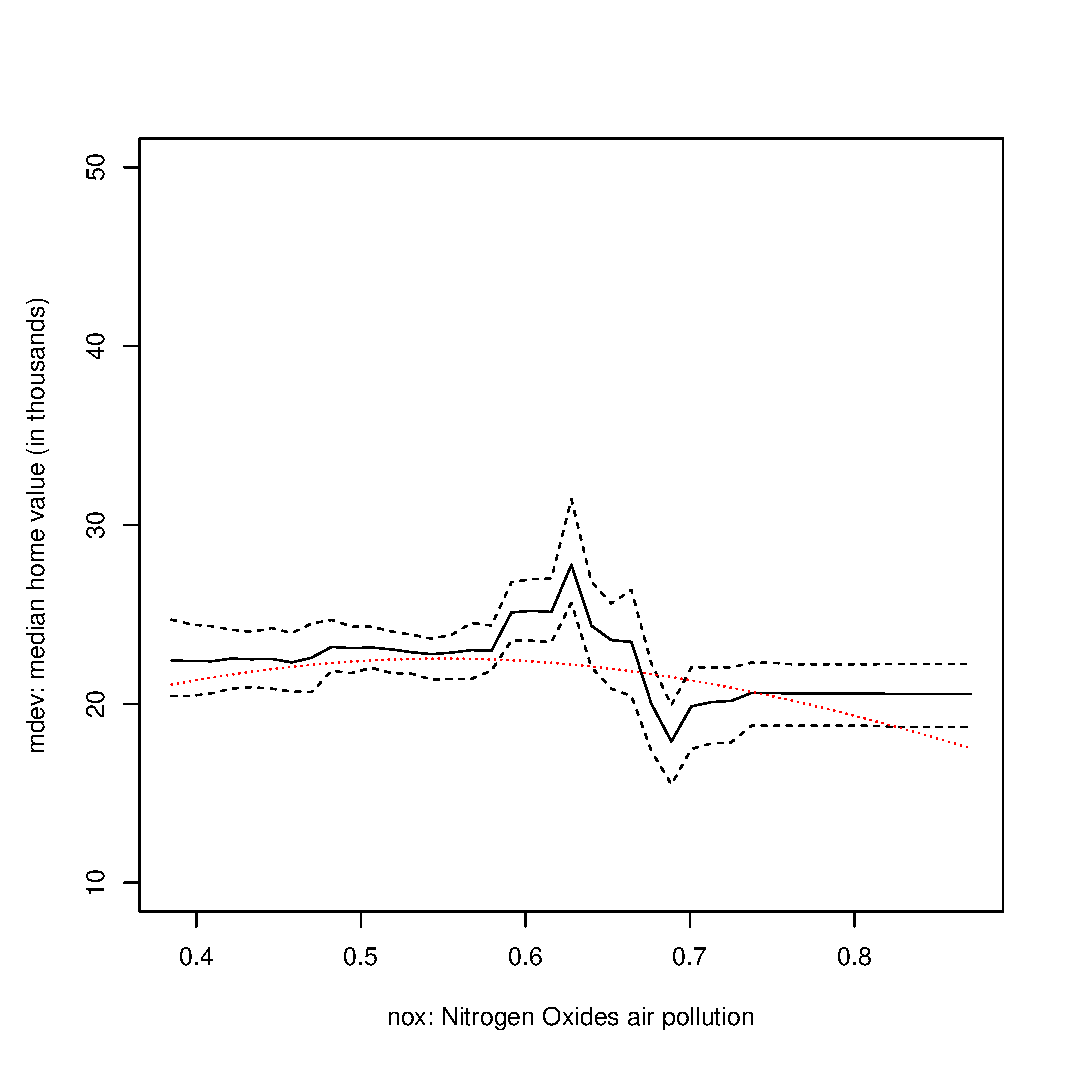
\includegraphics{figures/nox.eps}
\end{center}
\caption{\label{nox}The Boston housing data was compiled from the 1970
  US Census where each observation represents a Census tract in Boston
  with owner-occupied homes. For each tract, we have the median value
  of owner-occupied homes (in thousands of dollars), {\tt mdev}, and
  thirteen other covariates including a localized air pollution
  estimate, the concentration of nitrogen oxides {\tt nox}, which is
  our primary interest.  We summarize the marginal effect of {\tt nox}
  on {\tt mdev} while aggregating over the other covariates with
  Friedman's partial dependence function.  The marginal estimate and
  its 95\% credible interval are shown.  The red line with short
  dashes comes from the linear regression model of \cite{HarrRubi78}
  where a quadratic effect of {\tt nox} with respect to the logarithm
  of {\tt mdev} is assumed.}
\end{figure}

\section{Dichotomous, categorical and survival outcomes}
\label{gbart}

Dichotomous outcomes can be handled with either a probit or a logit
link function as in other Bayesian regression models.  For probit,
typically, the \cite{AlbeChib93} technique is employed while for the
logit link there are a few common alternatives
\citep{HolmHeld06,FruhFruh10,GramPols12}.  There are several
techniques for categorical outcomes as well; see
\citep{AlbeChib93,McCuRoss94,McCuRoss00,FruhFruh10,KindWang16,Murr17}.
For survival analysis, the approach of \textbf{Discrete Survival-time
  Models} \citep{Fahr14} can be used to turn the problem into a
dichotomous outcome (with either the probit or logit link)
\citep{SparLoga16} without resorting to precarious restrictive
assumptions such as those of the \textbf{Cox Proportional Hazard
  Model} \citep{CaiZeng14} or \textbf{Accelerated Failure-time Models}
\citep{Jame14}.  Similarly, the discrete survival-time approach is
applicable to recurrent events \citep{SparRein18} and competing risks
\citep{SparLoga19}.  For survival analysis with large data sets, you
can pair BART with Dirichlet Process Mixtures (see
\textbf{Nonparametric Bayes}, \cite{Duns17})
\citep{BonaBala11,HendLoui17}; however, you will need to make
assumptions like proportional hazards or accelerated failure-time.

\section{Recent developments and software implementations}
\label{final}

BART is still evolving as variants emerge for new purposes.
\cite{ZhanShi07} paired BART with a conditional autoregressive (CAR)
model for spatial data. Sequential BART is an adaptation to missing
value imputation \citep{XuDani16}.  \cite{PratChip17} adapt BART to
heteroscedastic data with two ensembles of trees: one that is BART and
another that is multiplicative (rather than additive like BART).
\cite{HahnMurr17} have extended BART to causal inference.
\cite{LineYang18} present what they call SoftBART which creates smooth
BART functions.  \cite{GeorLaud19} marry BART with Dirichlet Process
Mixtures to avoid the Normally distributed errors assumption.  Big
data sample sizes require developments which are helpful in using BART
with high perfomance computing frameworks such as the Message Passing
Interface \citep{WalkDong96,GabrFagg04}: two such approaches are the
Consensus MCMC \citep{PratChip14} and the Modified Likelihood
Inflating Sampling Algorithm \citep{EnteCrai18}.

Since BART is essentially a computational approach, software is
necessary for its use.  As of this writing, several R package
implementations of BART are available on the Comprehensive R Archive
Network (CRAN): {\it BART} \citep{McCuSpar19}, {\it bartMachine}
\citep{BleiKape14}, {\it BayesTree} \citep{ChipMcCu16} and {\it
  dbarts} \citep{DoriChip16}.

\begin{comment}
\MakeShortVerb{\|}

The first package was {\bf BayesTree} and it has been very influential
on packages that followed. It is written in C++ and supports
continuous and dichotomous outcomes.  Reported bugs will be fixed, but
no future improvements are planned. The second package, {\bf
  bartMachine}, is written in {java} \citep{KapeBlei16}.  It provides
advanced features like multi-threading, variable selection
\citep{BleiKape14}, a |predict| function, convergence diagnostics and
missing data handling.  The {R} to {java} interface is provided by the
{\bf rJava} \citep{Urba17} package which requires the Java Development
Kit (JDK) so we recommend {\bf bartMachine} for {java} users.

The third package, {\bf dbarts}, is also written in {C++}.  It is
designed as a drop-in replacement for {\bf BayesTree}.  Although, it
lacks multi-threading, the {\bf dbarts} serial implementation is the
fastest, therefore, it is preferable when multi-threading is
unavailable such as on Windows.  The last package, {\bf BART}, is
written in {C++}.  The {C++} interface to {R} is provided by the {\bf
  Rcpp} package \citep{EddeFran11} which seamlessly passes object
references from {R} to {C++} (and vice versa) as well as providing
direct accesss to the {R} random number generator. {\bf BART} provides
advanced features like multi-threading, variable selection
\citep{Line16}, a |predict| function, convergence diagnostics and
missing data handling.  It is the only BART package to support
continuous, dichotmous, categorical and time-to-event outcomes
\citep{SparLoga16} including recurrent events \citep{SparRein18} and
competing risks \citep{SparLoga19}.
\end{comment}

\section*{Related Articles}

\textbf{Accelerated Failure-time Models; Classification and Regression
  Tree Methods; Cox Proportional Hazard Model; Discrete Survival-time
  Models; Markov Chain Monte Carlo (MCMC, Metropolis-Hastings, Gibbs
  Sampling); Nonparametric Bayes; Overfitting (Overtraining);
  Regression Trees; Tree-structured Statistical Methods.}

%\bibliographystyle{plainnat}
\bibliographystyle{wb_stat}
\bibliography{bart.bib}

\end{document}

